\documentclass{article} % For LaTeX2e
\usepackage{nips14submit_e,times}
\usepackage{hyperref}
\usepackage{url}
\usepackage{amsmath}
\usepackage{amsfonts}
\usepackage{graphicx}
\usepackage{bibentry,natbib}

%\documentstyle[nips14submit_09,times,art10]{article} % For LaTeX 2.09


\title{ECE285 Project Progress Report: High Speed Imaging with Compressed Sensing}


\author{
Yingwei Li*, Huan Hu* \\
\AND huh015@eng.ucsd.edu
}

% The \author macro works with any number of authors. There are two commands
% used to separate the names and addresses of multiple authors: \And and \AND.
%
% Using \And between authors leaves it to \LaTeX{} to determine where to break
% the lines. Using \AND forces a linebreak at that point. So, if \LaTeX{}
% puts 3 of 4 authors names on the first line, and the last on the second
% line, try using \AND instead of \And before the third author name.

\newcommand{\fix}{\marginpar{FIX}}
\newcommand{\new}{\marginpar{NEW}}

\nipsfinalcopy % Uncomment for camera-ready version

\begin{document}


\maketitle

\begin{abstract}
In this course project, we plan to build a mathematical model for high speed imaging system with compressed sensing. Due to the sparseness of the underlying image, compressed sensing can be applied in the image reconstruction. We improve our design step by step by reviewing existing Compressive Imaging systems. We'll conduct simulations for a full-functioning imaging system and analyze the results for further improvements.
\end{abstract}

\section{Compressive Imaging v.s. Traditional Image Compression} There is an extensive body of literature on image compression, but the central concept is straightforward: we transform the image into an appropriate basis and then code only the important expansion coefficients. Natural images are inherently sparse under proper transforms as shown in figure~\ref{fig:naturalSparse}. The crux is finding a good transform, a problem which has been studied extensively from both a theoretical and practical standpoint. The most notable product of this research is the wavelet transform; switching from sinusoid-based representations to wavelets marked a watershed in image compression, and is the essential difference between the classical JPEG and modern JPEG-2000 standards.  In traditional image compression techniques, often, the image decoding stage is relatively simple, e.g. solving a least square problem.
%TOFIG
\begin{figure}[!h]
\centering
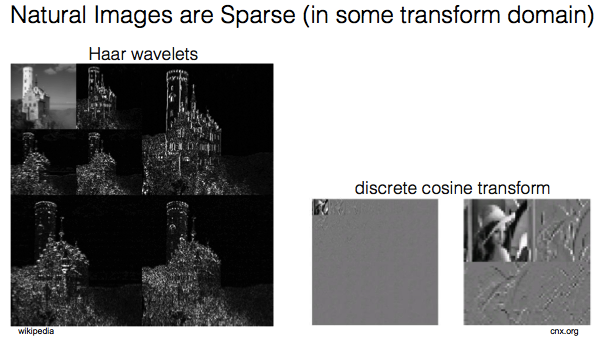
\includegraphics[width=3.5in]{naturalSparse.png}
\caption{natural images are sparse in transfer domain }
\label{fig:naturalSparse}
\end{figure}

In sum, traditional compression requires first Nyquist sampling of original image and then do compression by encoding in proper domain. This can be summarized as a procedure of "sample, process, keep the important information, and throw away the rest". 

As opposed to traditional image compression, Compressive Imaging does the compression at the data acquisition step. This reduces the data throughput right from the start of the system. In addition to image compression, in some cases, due to practical limitations such as time constraint as in MRI\cite{lustig2007sparse}, energy constraint as in wireless sensing network and other physical limitations as in our system, we'll have to resort to compressive sensing techniques in order to have high quality images under these constraints. 

In the following chapters, we first review several sparse imaging systems in the literature(chapter 2), with an emphasis on the image recovery problem formulation ,design of sensing matrix and algorithms to solve recovery problem. And in chapter 3, we describes our proposed system for high-speed nanometer scale imaging and experimental results. Since our system is under heavy experiment and design iteration, we list the possible future steps prior to our final fabrication.

\section{Compressive Imaging Literature Review}
We review a few papers related to compressive imaging systems. In particular, we're interested in the recovery problem formulation , sensing matrix design and algorithms to solve recovery problem.
\subsection{SparseMRI}
Magnetic resonance imaging (MRI) is a medical imaging technique used in radiology to investigate the anatomy and physiology of the body in both health and disease\cite{wiki:MRI}. The image system can sample the 2D Fourier transform(widely termed as \textbf{k-space}\cite{twieg1983k} in MRI literature) of the image to be reconstructed. If the k-space is full, the recovery procedure is almost trivial. However, the time requirement prohibits a fully sampled k-space. Hence, Compressive Imaging can be applied to reconstruct MR image with only few measurements.
\subsubsection{image recovery problem formulation}
\cite{lustig2007sparse} introduces a method for fast MRI. Instead of sampling the whole k-space, SparseMRI samples a collection of random points in k-space. This is equivalent to have a measurement matrix as random partial DFT matrix. The sparsity assumption can be made in either the imaging space or wavelet space.  The working flow is shown in figure~\ref{fig:sparseMRIFlow}.
%TOFIG
\begin{figure}[!h]
\centering
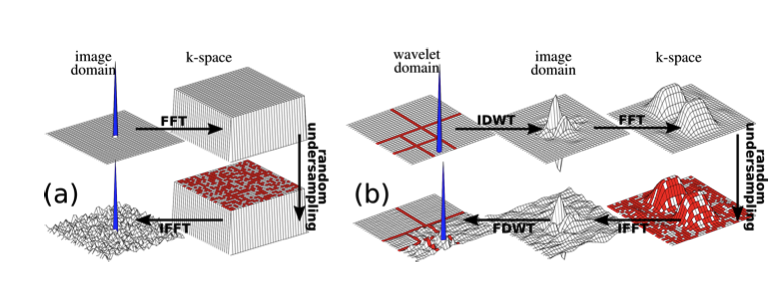
\includegraphics[width=3.5in]{sparseMRIFlow.png}
\caption{spareMRI workflow (a) The PSF of random 2D k-space undersampling. (b) The wavelet TPSF of random 2D Fourier undersampling. FDWT and IDWT stand for forward and inverse discrete wavelet transform. Wavelet coefficients are band-pass filters and have limited support both in space and frequency. Random k-space undersampling results in incoherent interference in the wavelet domain. The interference spreads mostly within the wavelet coefficients of the same scale and orientation.}
\label{fig:sparseMRIFlow}
\end{figure}


More specifically, we need to solve the inverse problem:
\begin{align*}
&b=F_u x \\
&s.j.~ \alpha=\Phi x,\alpha~is~sparse
\end{align*}
where A is the random partial DFT matrix and $\Phi$ is the domain where the image is sparse(can be either $I$ or the wavelet matrix).

This inverse problem can be solved with guarantee by L1 minimization since partial DFT matrix satisfy RIP conditions. That is,
\begin{align}
x^*&=\underset{x} {\mathrm{argmin}}~|\Phi x|_1 \\ 
\notag &s.j. ~|b-F_u x|_2<\epsilon
\label{eq:L1}
\end{align}
One thing that's particular interesting to our project is that, changing the L1 objective function to \textbf{Total Variation (TV)} is closed related to sparsity assumption in wavelet space. More generally, even if the sparsity domain is not wavelet space, a TV term can also be added to enforce smoothness. We hope this is useful in our imaging system. With the TV term, the reconstruction problem now becomes:

\begin{align}
x^*&=\underset{x} {\mathrm{argmin}}~ |\Phi x|_1+\lambda TV(x) \\
\notag &s.j.~|b-F_ux|_2<\epsilon\\
\notag &\text{where}~TV(x)=|D(x)|, D(x) ~\text{is the discrete differential operator}. 
\label{eq:TV}
\end{align}

\subsubsection{discussions about sensing matrix}
As the paper discusses, the validity of compressive sensing in MRI largely depends on the nice property of the sensing matrix, which is partial DFT matrix. In their discussion, an intuitive heuristic guideline for evaluation of the sensing matrix is defined. As we desire \textbf{incoherent artifacts caused by undersampling}, a natural measure would be the \textbf{Transform Point Spread Function(TPSF)} as defined in the paper, where
\begin{align}
TPSF(i;j)=e_j^* \Phi F_u^* F_u \Phi^* e_i
\end{align}

And we would like $TPSF(i;j)|_{i \neq j}$ as small as possible.Actually, this purpose is exactly the same as minimizing the mutual coherence of a matrix which is discussed in our early lectures. We know it can lead to sufficient conditions for exact recovery. 

Thus, we would like to experiment with minimization of mutual coherence of the sensing matrix in our imaging system, although we're given limited freedom of choice(the sensing matrix is related to the optical properties and layout of the materials in the system).

The paper also discusses a lot about the sampling strategy considering smooth sample trajectories due to hardware and physiological limitations. Moreover, their system also has a "calibration" step to correct phase misalignment, which is similar to our system.

\subsection{Single-Pixel Imaging}
\subsubsection{hardware architecture}
In \cite{duarte2008single}, the author describes a full-blown imaging system with only a single photon detector.  The system is mainly composed of biconvex lenses, a DMD(digital micromirror device) spatial light modulator , a single photon detector and a A/D converter. This whole architecture is essentially a optical computer shown in figure~\ref{fig:singlePixFlow}. Since the DMD is programmable, the system can get $M$ random measurement of the scene by generating different patterns and take the inner product with the image. With sufficiently large number of measurement($M= O(K log(N/K))$), we're guaranteed to have exact imaging result. 

\begin{figure}[!h]
\centering
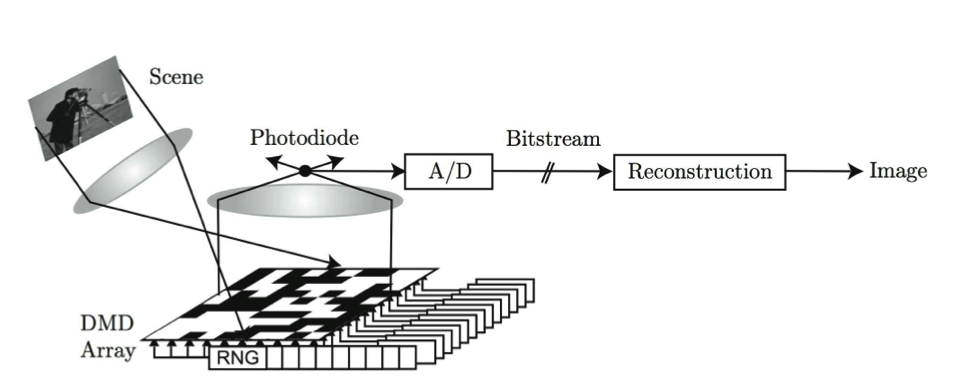
\includegraphics[width=3.5in]{singlePixFlow.png}
\caption{Single-Pixel Imaging workflow }
\label{fig:singlePixFlow}
\end{figure}

\subsubsection{recovery problem formulation}
For different mirror configurations, the system will have different measurement pattern $\phi_i$, the single photon detector will detect the modulated scalar signal $y_i$.  Concatenating all the measurements, we have the measurement equation:
\begin{align*}
y = \Phi x 
\end{align*}
where y is an $M \times 1$ column vector and the measurement basis matrix $\Phi$ is $M \times N$ with each row a basis vector $\phi_m$.

The recovery problem formulation is very similar to MRI case shown in equation \ref{eq:L1}, except with a different sensing matrix. Also, the paper also mentioned using the TV formulation in addition to L1 minimization as in equation \ref{eq:TV}.
\subsubsection{sensing matrix design}
The system uses random rows of 0/1 Walsh matrix as the sensing matrix. But the paper also suggests Hadamard or noiselet transform\cite{coifman2001noiselets}. These are all sampled rows from a deterministic matrix instead of the i.i.d Gaussian case discussed in our lectures.
\subsubsection{image classification by smashing filter}
The paper demonstrates one interesting experiment of image classification. They argue that the naive approach would first reconstruct the full image and then do classification in the original image space $R^n$. The smashed filter exploits a recent result that the structure of a smooth K-dimensional manifold in $R^N$ is preserved with high probability under a random projection to the lower dimensional space $R^M$ as long as $M = O (K log N )$ (note this is quite similar to the guarantee of exact recovery of sparse signal although here it's a subspace). With this guarantee, the smashed filter performs all the operations on the measurements directly without recovery of the full image.

The paper shows that with more measurements, the accuracy of classification by smashed filter increases, which satisfies our intuition.

\subsection{CI by CMOS Separable Image Sensor}
\subsubsection{hardware architecture}
\cite{robucci2010compressive} discusses the application of a computational image sensor, capable of performing separable 2-D transforms on images in the analog domain, to compressive imaging. For separable 2-D transforms, the computation could be simplified to inner products. In their system, the inner products are computed using a computational focal-plane and a computational analog vector-matrix multiplier.
 
The image sensor design was implemented on a $22.75~mm^2$ die in a standard $.35~\mu m$ CMOS process. The resolution is $256 \times 256$ with a pixel size of $8 \mu m \times 8 \mu m$.

A flowchart of the system is shown in figure~\ref{fig:sepFlow}.
%TOFIG
\begin{figure}[!h]
\centering
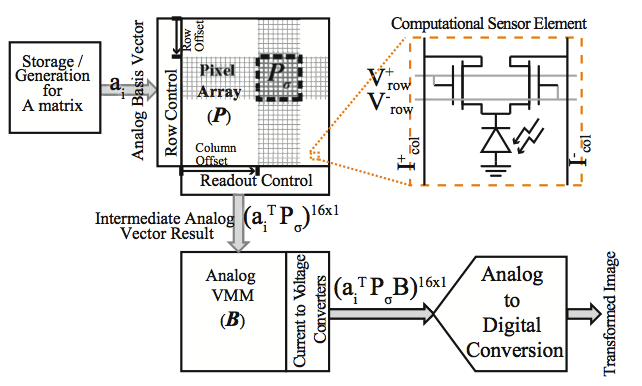
\includegraphics[width=3.5in]{sepFlow.png}
\caption{CI by CMOS Separable Image Sensor workflow }
\label{fig:sepFlow}
\end{figure}

\subsubsection{recovery problem formulation}
The fundamental capability of this image sensor can be described as a matrix transform: $Y_\sigma = A^TP_\sigma B$, where A and B are transformation matrices, Y is the output, P is the image, and the subscript $\sigma$ denotes the selected $16\times16$ pixel sub-region of the image under transform. This is essentially a compressive sensing stage, since the transformation given by $A$ and $B$ could be a subset of the DCT coefficients. 

The imaging system takes advantage of the separable property of the DCT transform, thus simplifies the design for the CMOS circuits and also the sensing time. The recovery problem formulation in the paper is as follows:
\begin{align}
x^*&=\underset{x} {\mathrm{argmin}}~TV(x)\\
&s.j~||\Phi x - y||_2 \leq \epsilon
\end{align}
where $x \in \mathbb{R}^{n^2}$ $\Phi$ is of size $m \times n^2$, the partial DCT matrix and $y$ is the $m$ vector containing the measurements.
\subsubsection{sensing matrix design}
As the system only works for the case when the transform is separable, the sensing matrix can not be iid gaussian matrix. In the paper, they discuss both the DCT matrix and the noiselet matrix as shown in figure~\ref{fig:DCTnoiselet}, since both of them are separable. 
%TOFIG
\begin{figure}[!h]
\centering
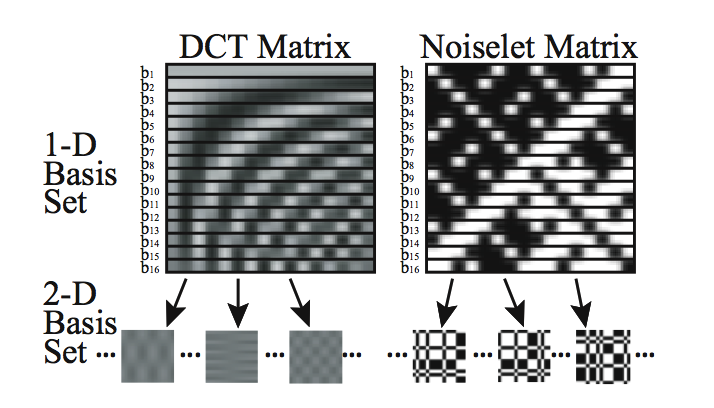
\includegraphics[width=3.5in]{DCTandNoiselet.png}
\caption{DCT matrix and noiselet matrix }
\label{fig:DCTnoiselet}
\end{figure}

However, as their experiment results shows, noiselet matrix works better in practice. The reason this occurs is that: the inner products with the different DCT basis functions are generally non-uniform, since most of the energy in images lies in the low frequency components. The noiselets basis are decorrelated with most image features and with reconstruction basis functions, making each noiselet basis function statistically as significant as any other.

\section{Our High-speed Nanometer Compressive Imaging System}
\subsection{Hardware Architecture}
[a brief intro to the sensing system ]
\subsection{}
\subsection{}
\subsection{different design of sensing matrix $A$}
Based on the underlying theory of photonics, we simulate two settings of the sensing matrix.($A1$ and $A2$) (we leave out the technical details here). 
Both $A1$ and $A2$ are generated by randomly placing light sources on our optical material hence has some randomness(the exact distribution is unknown due to complex physical interaction). An example of $A1$ and $A2$ is shown in Figure 1 and Figure 2 respectively.

 For $A1$, the sensing structure is relatively simpler and can only sensing one dimension of the underlying image(i.e. determine if \textit{any} pixel in a column is non-zero). figure[??] shows an example of L1 recovery result.
 
From our experiment, with $A1$ of size $30 \times 80$, sparsity 10,image size 80, the system is quite reliable to recover the original image. This is a promising result.

For $A2$, we include more complex layout strategy for the light sources hence resulting sensing matrix that can sense 2-D images. Figure 2 shows an example of the recovery result.

We compare two different algorithms for solving the L1 minimization problem. One provided by \cite{koh2007interior} which is a l1-Regularized Least Squares method. The other is termed as \textbf{smoothed L0 norm (SL0)}\cite{mohimani2008complex} which tries to directly minimize the L0 norm with a approximation function (in our experiment SL0 performs better).

From our experiment, with $A2$ of size $160 \times 400$, sparsity 20, image size $20 \times 20$, the system can successfully recover the original image. 

%\begin{figure}[!t]
%\centering
%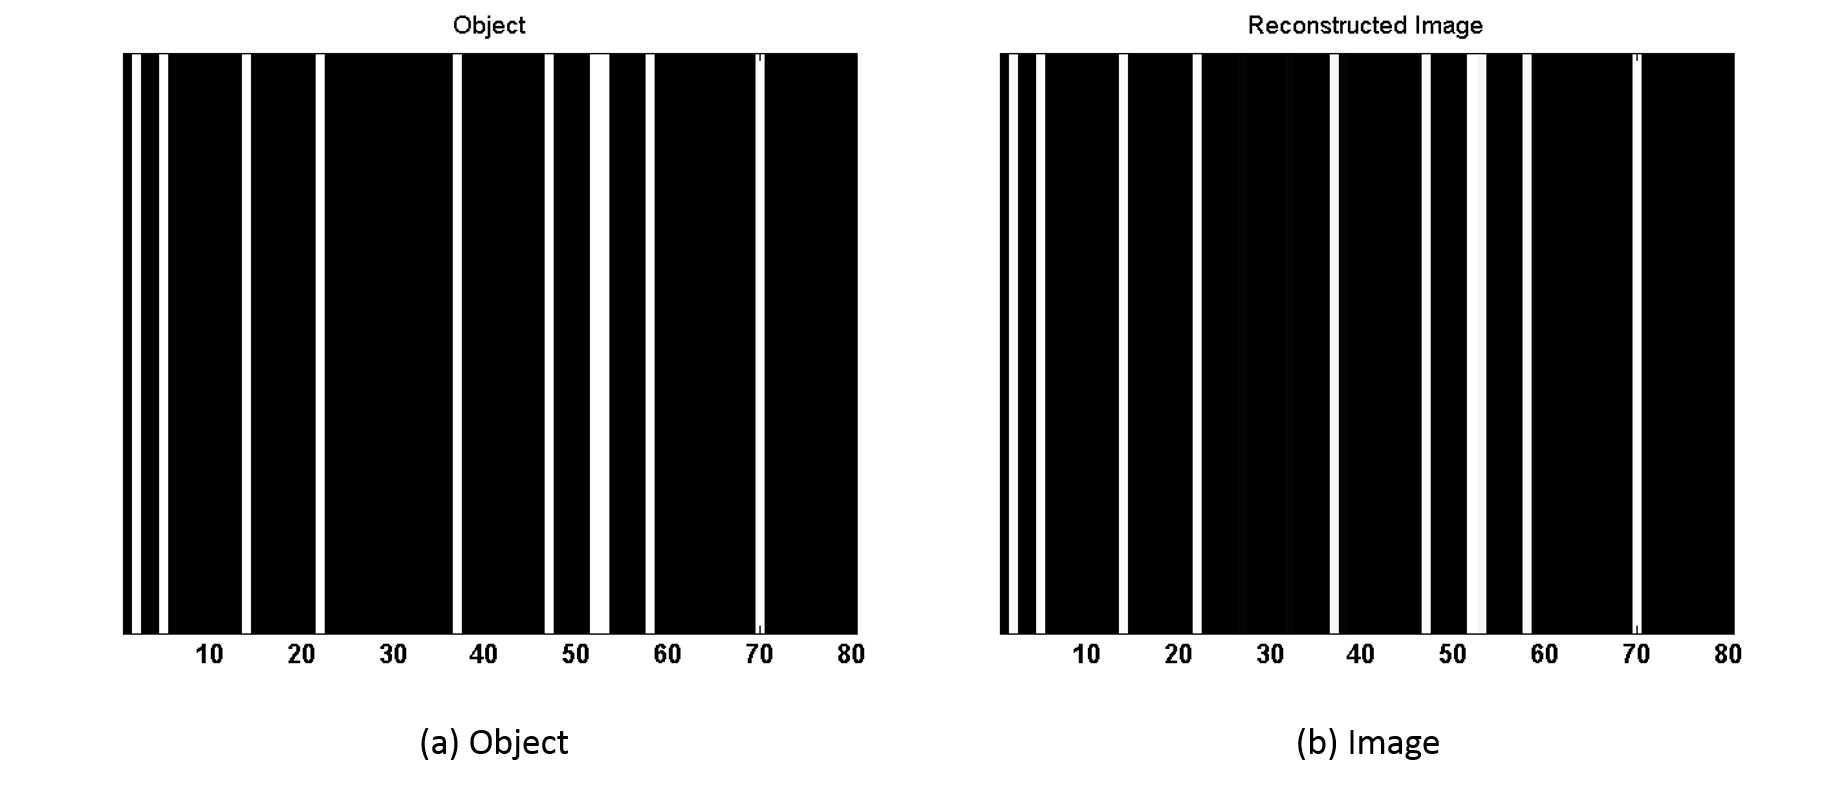
\includegraphics[width=5in]{5.png}
%% where an .eps filename suffix will be assumed under latex,
%% and a .pdf suffix will be assumed for pdflatex; or what has been declared
%% via \DeclareGraphicsExtensions.
%\caption{A1: 1D imaging computational experiment }
%\end{figure}
%
%\begin{figure}[!t]
%\centering
%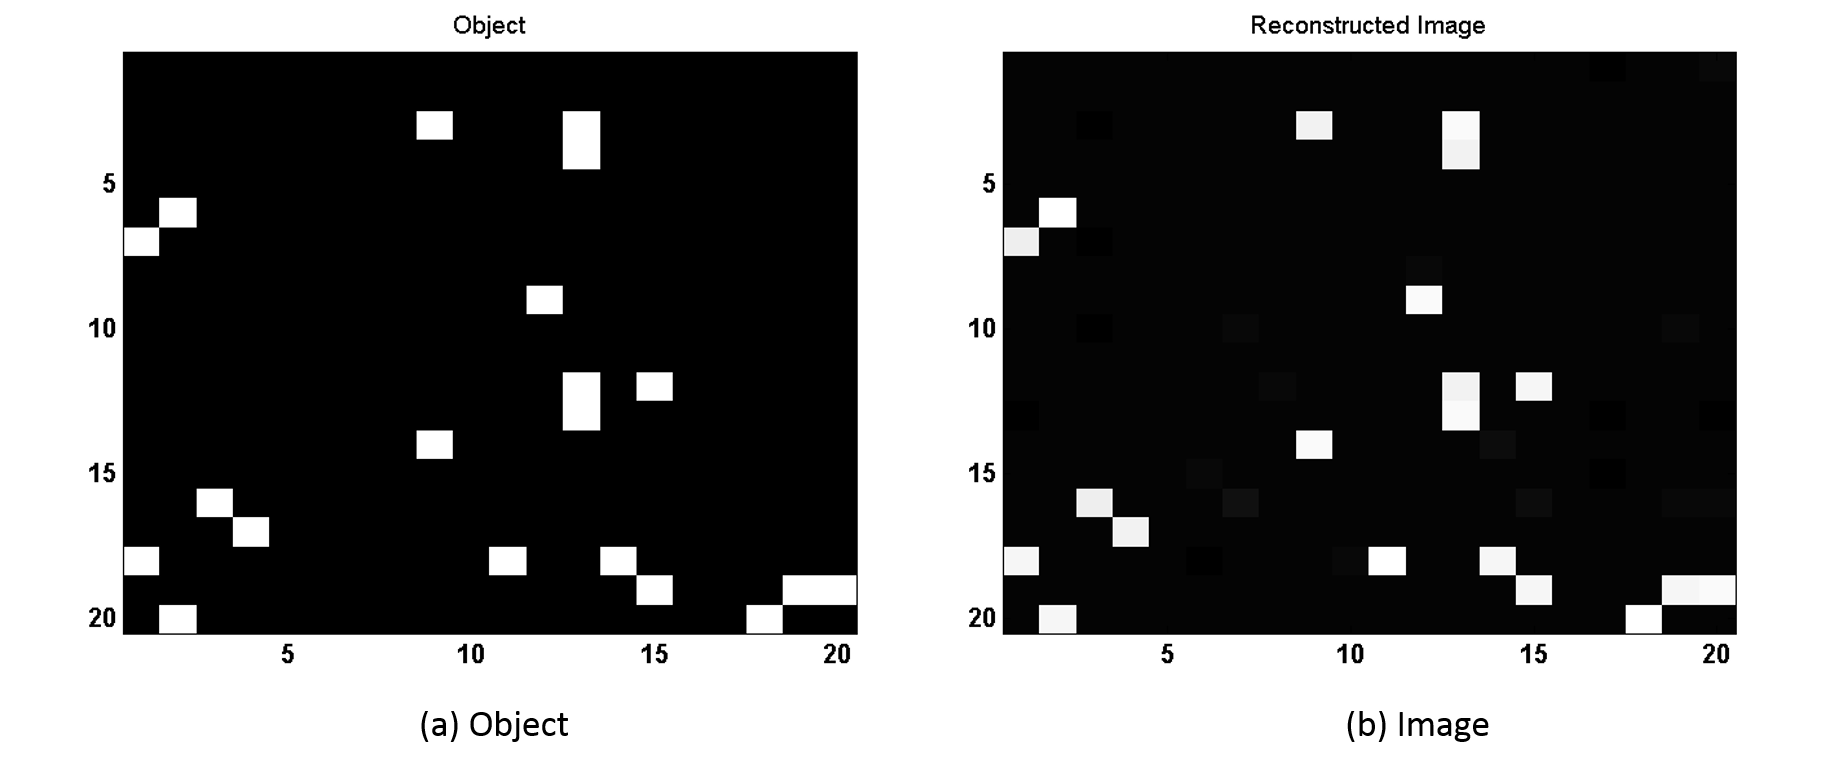
\includegraphics[width=5in]{6.png}
%% where an .eps filename suffix will be assumed under latex,
%% and a .pdf suffix will be assumed for pdflatex; or what has been declared
%% via \DeclareGraphicsExtensions.
%\caption{A2: 2D imaging computational experiment }
%\end{figure}

\section{Future Work}
The proposed method for high-speed nanometer imaging requires design considerations both from optics and signal processing aspects. For future steps, we would like to investigate the following subjects:
\begin{enumerate}
\item Refine physical design to increase measurement number $M$.
	Since at the end of the day, the most critical limitation is the measurement number. With more measurements, we'll certainly get better results.
\item To solve sparse recovery problems, a lot of solvers are available online, each with different approaches to relax the original L0 problem. We'll continue to evaluate their performance with respect to imaging quality in our system and hopefully will find the optimal one for our purpose.
\item In some cases, we know the image is composed of several sparse blocks, each with a known shape. In this case, the assumption of \textbf{block sparsity} is more proper. A nice way to incorporate this prior information is expected to improve the imaging result.
\end{enumerate}

\bibliographystyle{unsrt}
\bibliography{ref}

%\vspace*{3\baselineskip}
%
%\small{
%[1] Willett R M, Marcia R F, \&Nichols J M. Compressed sensing for practical optical imaging systems: a tutorial[J]. {\it Optical Engineering}, 2011, 50(7): 072601-072601-13.
%
%[2] Lustig, Michael, David Donoho, \& John M. Pauly. "Sparse MRI: The application of compressed sensing for rapid MR imaging." {\it Magnetic resonance in medicine 58.6 (2007)}: 1182-1195.
%
%[3] Duarte M F, Davenport M A, \&Takhar D, et al. Single-pixel imaging via compressive sampling[J]. {\it IEEE Signal Processing Magazine}, 2008, 25(2): 83.
%
%[4] Koh K, Kim S J, Boyd S P. An interior-point method for large-scale l1-regularized logistic regression[J]. Journal of Machine learning research, 2007, 8(8): 1519-1555.
%
%[5] Mohimani, G. Hosein, Massoud Babaie-Zadeh, \& Christian Jutten. Complex-valued sparse representation based on smoothed L0 norm. {\it Acoustics, Speech and Signal Processing, 2008. ICASSP 2008. IEEE International Conference on.} IEEE, 2008.

%[1] Alexander, J.A. \& Mozer, M.C. (1995) Template-based algorithms
%for connectionist rule extraction. In G. Tesauro, D. S. Touretzky
%and T.K. Leen (eds.), {\it Advances in Neural Information Processing
%Systems 7}, pp. 609-616. Cambridge, MA: MIT Press.
%
%[2] Bower, J.M. \& Beeman, D. (1995) {\it The Book of GENESIS: Exploring
%Realistic Neural Models with the GEneral NEural SImulation System.}
%New York: TELOS/Springer-Verlag.
%
%[3] Hasselmo, M.E., Schnell, E. \& Barkai, E. (1995) Dynamics of learning
%and recall at excitatory recurrent synapses and cholinergic modulation
%in rat hippocampal region CA3. {\it Journal of Neuroscience}
%{\bf 15}(7):5249-5262.
%}

\end{document}
